%=================================
% Type de document
%=================================
\documentclass[12pt,a4paper]{report}

%=================================
% PRÉAMBULE - PACKAGES
\usepackage{caption}
\usepackage{rotating}
\usepackage{lipsum}   % For dummy text if needed
\usepackage{setspace} % For line spacing control
\usepackage[hyphens]{url}
\usepackage{hyperref}
\urlstyle{same}
%=================================
\usepackage{float}

%1. Traitement des caractères spéciaux
\usepackage[T1]{fontenc}
\usepackage[utf8]{inputenc}

%2. Gestion du français et sommaire local par chapitre


%3. Mise en page et graphiques
\usepackage[top=2.5cm, bottom=2.5cm, left=2.5cm, right=2.5cm]{geometry}
\usepackage[pdftex]{graphicx} 
\usepackage{float} 
\usepackage{url}
\usepackage{pdflscape}  % Pour les pages en orientation paysage

%4. Style du texte et typographie
\usepackage{pslatex} 
\usepackage{setspace} 
\usepackage{enumerate}
\usepackage{array}
% 2. Gestion du français et sommaire local par chapitre
\usepackage[french]{babel}
\addto\captionsfrench{\renewcommand{\tablename}{Tableau}}

\usepackage[french]{minitoc} 

%\usepackage{caption}    
\usepackage{longtable}
\usepackage{multirow}
\usepackage{enumitem}
\usepackage[font=small,labelfont=bf]{caption}
\onehalfspacing 

%5. Espace entre paragraphes
\setlength{\parskip}{10pt}

%6. Style de chapitres
\usepackage[Glenn]{fncychap}

% Hyperref devrait être chargé après les autres packages
\usepackage[colorlinks=true, linkcolor=blue, citecolor=green, urlcolor=magenta]{hyperref}
\usepackage[final]{pdfpages} 

%7. En-têtes et pieds de page
\usepackage{fancyhdr}
\pagestyle{fancy}
\fancyhf{}
\fancyhead[LE,RO]{\nouppercase{\leftmark}}  
\fancyfoot[LE,RO]{\thepage} 
\fancyfoot[L]{Projet de Fin d'Études - ENOVA ROBOTICS}
\renewcommand{\headrulewidth}{0.4pt}
\renewcommand{\footrulewidth}{0.4pt}

%8. Configurations supplémentaires
\setcounter{secnumdepth}{4}
\setcounter{tocdepth}{2}

% Initialiser minitoc
\dominitoc

%=================================
% DOCUMENT PRINCIPAL
%=================================
\begin{document}

%===== Page de garde
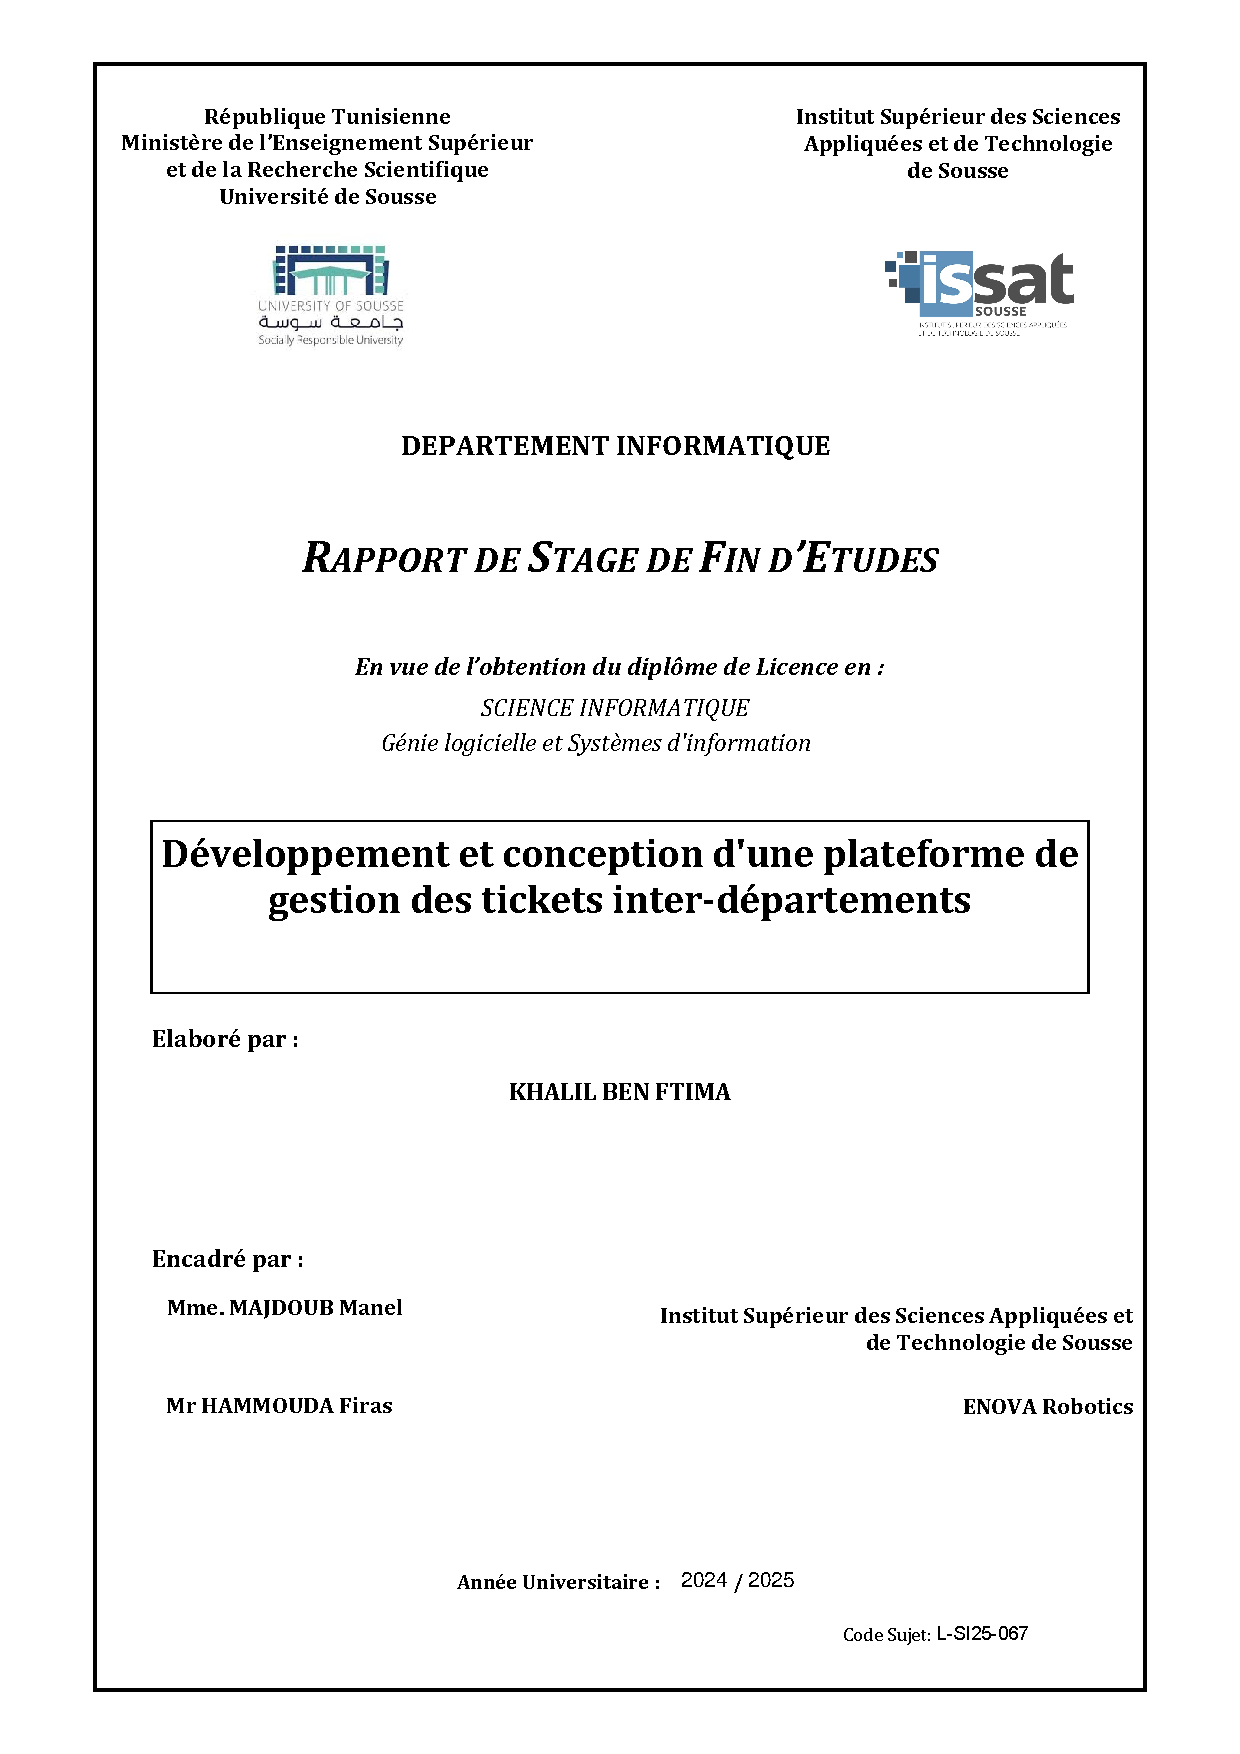
\includepdf{PageDeGardePFE.pdf}

%===== Passage à la numérotation romaine pour les pages préliminaires
\pagenumbering{roman}

%===== Dédicace
\cleardoublepage
\chapter*{Dédicace}
\addcontentsline{toc}{chapter}{Dédicace}
\markboth{Dédicace}{}
% TODO: Rédiger la dédicace
% La dédicace est généralement une page personnelle où vous dédiquez votre travail à quelques personnes importantes.

[CONTENU À REMPLIR: Dédicace personnelle]

% Exemple de structure de dédicace:
% 
% Je dédie ce travail à :
% 
% [Personne 1] pour son soutien constant et ses encouragements...
% 
% [Personne 2] pour ses conseils avisés et son expertise...
% 
% [Personne 3] pour sa patience et sa compréhension...
% 
% Et à tous ceux qui ont contribué de près ou de loin à la réalisation de ce projet.


%===== Remerciements
\cleardoublepage
\chapter*{Remerciements}
\addcontentsline{toc}{chapter}{Remerciements}
\markboth{Remerciements}{}
% TODO: Rédiger les remerciements
% Les remerciements doivent exprimer votre gratitude aux personnes et institutions
% qui ont contribué à votre travail (encadrants, superviseurs, collègues, etc.)

[CONTENU À REMPLIR: Remerciements]

% Exemple de structure de remerciements:
% 
% Je tiens à exprimer mes plus sincères remerciements à :
% 
% [Encadrant/Superviseur] pour son encadrement, ses conseils précieux et sa disponibilité tout au long de ce projet...
% 
% [Entreprise/Institution] et ses équipes pour m'avoir accueilli et offert l'opportunité de réaliser ce projet...
% 
% [Personne/Équipe] pour leur aide technique et leurs suggestions constructives...
% 
% [Professeurs/Mentors] de [Université/École] pour la formation reçue...
% 
% Et enfin, je remercie [Famille/Amis] pour leur soutien moral et leurs encouragements constants.


%===== Table des matières et listes
\cleardoublepage
\tableofcontents

\cleardoublepage
\listoffigures

\cleardoublepage
\listoftables

%===== Passage à la numérotation arabe pour le corps du rapport
\cleardoublepage
\pagenumbering{arabic}

%===== Introduction générale
\cleardoublepage
\chapter*{Introduction Générale}
\addcontentsline{toc}{chapter}{Introduction Générale}
\markboth{Introduction Générale}{}
%définir l'entête de ce chapitre 
\markboth{Introduction Générale}{}

Le secteur de la gestion des ressources humaines connaît aujourd'hui une transformation profonde, portée par les avancées rapides des technologies numériques. Les organisations, qu'elles soient de grande envergure ou de taille intermédiaire, sont confrontées à des défis croissants en matière d'administration du personnel, de suivi des performances et de pilotage stratégique des ressources humaines. Dans ce contexte en perpétuelle mutation, la capacité à centraliser les données, à automatiser les processus et à intégrer des outils intelligents est devenue un facteur déterminant de compétitivité et d'efficacité organisationnelle.

Les PME et ETI souffrent particulièrement de l'absence de solutions RH à la fois complètes, flexibles et accessibles. Les systèmes existants sur le marché présentent soit une complexité technique et des coûts prohibitifs inadaptés aux petites structures, soit des fonctionnalités trop limitées pour répondre pleinement aux besoins métier. Face à cette lacune identifiée, une décision stratégique a été prise de concevoir et de développer une plateforme intégrée de gestion des ressources humaines dénommée SMART RH 4.0, capable d'offrir une expérience utilisateur optimale et de permettre aux organisations d'accéder facilement à une suite complète d'outils et de services RH.

C'est dans ce contexte que s'inscrit ce projet de fin d'études, réalisé au sein de l'entreprise dans le cadre de l'obtention du diplôme national d'ingénieur en génie logiciel. Ce stage représente également une opportunité de mettre en pratique les connaissances théoriques acquises tout au long du cursus académique, de consolider les compétences techniques et de se confronter aux réalités du monde professionnel en tant que développeur et architecte de solutions d'entreprise.

Notre mission consiste à concevoir et développer la plateforme SMART RH 4.0, en visant une expérience utilisateur fluide et intuitive, tout en permettant aux organisations de bénéficier d'une gamme étendue de services RH intégrés, couvrant la gestion des employés, le suivi des performances, la gestion de la paie ainsi que le recrutement.

Ce rapport retrace les différentes étapes de réalisation du projet. Il est structuré en quatre chapitres, répartis comme suit :

\begin{itemize}
    \item Le premier chapitre, intitulé « Cadre général du projet », présente l'organisme d'accueil, expose le contexte et les enjeux du projet, détaille la mission confiée, ainsi que la méthodologie de travail adoptée pour sa réalisation.
    
    \item Le deuxième chapitre, « Analyse et spécification des besoins », se penche sur les étapes cruciales de la démarche à suivre pour comprendre les exigences fonctionnelles et non fonctionnelles de la plateforme SMART RH 4.0. Il identifie également les acteurs clés impliqués et présente de manière claire les diagrammes de cas d'utilisation ainsi que le diagramme de classes, permettant une vision d'ensemble du système.
    
    \item Le troisième chapitre, « Aperçu conceptuel », approfondit la planification en détaillant les diagrammes de cas d'utilisation pour chaque fonctionnalité spécifique, les diagrammes de séquence, ainsi qu'une analyse de la conception architecturale et de la structure des données retenue pour notre solution.
    
    \item Enfin, le quatrième chapitre, « Réalisation », est consacré à l'étude technique du projet. Il spécifie les technologies et les outils utilisés, et présente la réalisation concrète des modules clés de la plateforme SMART RH 4.0, accompagnée de captures d'écran représentatives des interfaces développées tout au long de la période de stage.
\end{itemize}

Ce rapport se conclut par une synthèse récapitulant le travail accompli, les résultats obtenus, ainsi que les perspectives d'évolution et d'amélioration envisagées pour la plateforme SMART RH 4.0.


%===== Chapitres
\cleardoublepage
\chapter{Présentation du cadre de projet}
\section*{Introduction}
\addcontentsline{toc}{section}{Introduction}

Dans ce premier chapitre, nous présentons le cadre général du projet. Tout d'abord, nous introduisons l'entreprise d'accueil, ses services et les technologies appropriées. Ensuite, nous comparons notre solution à celles déjà disponibles sur le marché. Enfin, nous définissons la méthodologie de développement adoptée.

Ce chapitre pose les bases en fournissant une vue d'ensemble du projet, en décrivant l'entreprise hôte, en analysant l'existant et en spécifiant les besoins fonctionnels et non fonctionnels.

\section{Contexte général du projet}

\subsection{Cadre du projet}

Le stage constitue une opportunité précieuse pour enrichir nos connaissances académiques et acquérir une expérience professionnelle concrète dans le domaine de l'informatique. Dans le cadre de l'obtention du diplôme national d'ingénieur en IoT \& Robotic Programming à l'EPI (École Pluridisciplinaire Internationale), nous avons réalisé un projet au sein de l'entreprise GOOD GOV IT Service \& Solution.

Ce projet consiste en le développement d'une plateforme intelligente, intitulée « Smart RH 4.0 », intégrant des technologies IoT et web, dédiée à la gestion des ressources humaines et à l'optimisation des processus de formation.

\subsection{Présentation de la société d'accueil : GOOD GOV IT}

« GOOD GOV IT Service \& Solution » est une entreprise spécialisée dans les technologies de l'information, orientée vers le développement de solutions innovantes et la transformation digitale des organisations. Présente principalement en Tunisie, elle accompagne ses clients dans la mise en place de systèmes intelligents intégrant des technologies modernes telles que le développement web, les applications mobiles et l'Internet des Objets (IoT).

À travers ses différentes expertises, l'entreprise propose des solutions adaptées aux besoins spécifiques de ses clients dans divers secteurs. Reconnue pour son engagement envers la qualité et l'innovation, « GOOD GOV IT Service \& Solution » se positionne comme un acteur dynamique dans le domaine des services numériques. Elle se spécialise notamment dans la conception de plateformes digitales, l'automatisation des processus et le développement de solutions technologiques avancées.

\subsection{Services}

GoodGovIT propose des services à forte valeur ajoutée, pensés pour répondre aux besoins spécifiques de chaque client, qu'il soit issu du secteur public ou privé :

\begin{itemize}
    \item \textbf{Développement sur mesure} : GoodGovIT développe des applications web, desktop et embarquées adaptées à tous les types de supports et de secteurs d'activité, en alliant performance, ergonomie et évolutivité.
    
    \item \textbf{Staffing \& Ressources humaines IT} : GoodGovIT met à disposition des ressources humaines hautement qualifiées dans des domaines technologiques variés, incluant le développement Fullstack, l'ingénierie Cloud, le développement mobile ainsi que l'analyse de données et la Business Intelligence.
    
    \item \textbf{GoodGovIT Academy} : GoodGovIT s'engage dans la montée en compétences des talents numériques à travers des cours en ligne flexibles, des bootcamps immersifs et des certifications reconnues, accompagnés d'un suivi personnalisé.
\end{itemize}

\section{Idée émergente et étude de l'existant}

\subsection{Idée émergente}

Dans un contexte marqué par l'essor de la transformation numérique, l'entreprise a entrepris une initiative stratégique visant à concevoir une plateforme RH intégrée. À travers le développement de la plateforme « SMART RH 4.0 », l'entreprise ambitionne d'offrir une expérience utilisateur optimale tout en consolidant sa position sur le marché des solutions RH.

L'objectif principal est de favoriser l'interaction entre les différents acteurs de l'entreprise, notamment les équipes RH, les responsables et les employés, tout en améliorant l'efficacité opérationnelle grâce à une application intégrée, intuitive et conviviale.

\subsection{Analyse de l'existant}

Une étude approfondie de l'existant est une étape essentielle avant d'entamer la réalisation de notre projet. L'analyse des solutions actuelles de gestion des ressources humaines nous permet d'avoir une vision globale du contexte et d'identifier les besoins réels des entreprises, ainsi que les limites des systèmes existants.

Actuellement, plusieurs solutions RH sont proposées sur le marché. Nous présentons ci-dessous trois exemples représentatifs de l'existant :

\textbf{SAP SuccessFactors} est une solution RH cloud de niveau entreprise développée par SAP. Elle offre une suite complète de modules couvrant la gestion des talents, le recrutement, la formation, la gestion de la paie et l'évaluation des performances. Conçue principalement pour les grandes organisations, elle se distingue par sa robustesse, sa richesse fonctionnelle et ses capacités d'intégration avec les autres produits SAP. Cependant, sa complexité de mise en œuvre et son coût élevé la rendent peu accessible aux PME.

\textbf{BambooHR} est une plateforme RH légère et intuitive, particulièrement appréciée des petites et moyennes entreprises. Elle propose des fonctionnalités essentielles telles que la gestion des dossiers employés, le suivi des absences, les processus d'intégration et le reporting RH basique. Son interface conviviale permet une prise en main rapide et un déploiement efficace. Néanmoins, elle présente des limites notables en matière de gestion de la paie, de personnalisation et de performance pour de grands volumes de données.

\textbf{Zoho People} est une solution RH cloud proposée par Zoho Corporation, adaptée aux entreprises de toutes tailles. Elle couvre la gestion des présences, des congés, des performances, des formations et de l'onboarding. Intégrée à l'écosystème Zoho, elle offre une bonne interopérabilité avec d'autres outils métier. Toutefois, ses workflows d'approbation restent peu flexibles et ses tableaux de bord analytiques manquent de profondeur pour un pilotage RH avancé.

Ces différentes solutions permettent généralement :

\begin{itemize}
    \item La gestion des informations des employés (dossiers, contrats, absences, etc.).
    \item Le suivi des processus de recrutement et d'intégration.
    \item La gestion des formations et des compétences.
    \item L'évaluation des performances des employés.
\end{itemize}

\subsection{Critique de l'existant}

En étudiant les solutions RH existantes, nous avons constaté qu'elles se limitent à des fonctionnalités basiques. Certaines fonctionnalités ne bénéficient pas d'une expérience utilisateur immersive et adaptée aux spécificités des besoins métier modernes.

Cette analyse comparative met en évidence les lacunes communes aux solutions existantes et justifie le besoin de développer une plateforme comme SMART RH 4.0, capable de répondre à l'ensemble de ces critères de manière intégrée, flexible et accessible.

\subsection{État de l'art}

Afin de proposer une solution complète et compétitive, nous avons étudié les meilleures pratiques du marché.

\subsubsection*{Workday (Leader de marché)}

\textbf{Points forts :}
\begin{itemize}
    \item Cloud-native et très sécurisé.
    \item Dashboards analytiques avancés.
    \item Intégrations nombreuses (200+ applications).
    \item Excellente expérience utilisateur.
\end{itemize}

\textbf{Points faibles :}
\begin{itemize}
    \item Coût très élevé (5 000€ à 50 000€/mois).
    \item Temps d'implémentation très long.
    \item Configuration complexe.
\end{itemize}

\subsubsection*{BambooHR (Solution légère populaire)}

\textbf{Points forts :}
\begin{itemize}
    \item Interface conviviale et intuitive.
    \item Bon rapport coût-performance.
    \item Déploiement rapide.
    \item Application mobile native bien développée.
\end{itemize}

\textbf{Points faibles :}
\begin{itemize}
    \item Fonctionnalités limitées en gestion de paie.
    \item Absence de véritable traçabilité d'audit.
    \item Personnalisation limitée.
    \item Performance limitée pour de grands volumes.
\end{itemize}

\subsubsection*{Microsoft Dynamics 365 Human Resources}

\textbf{Points forts :}
\begin{itemize}
    \item Intégration complète avec l'écosystème Microsoft.
    \item Extensibilité via Power Platform.
    \item Gestion complète de la paie et des avantages.
\end{itemize}

\textbf{Points faibles :}
\begin{itemize}
    \item Courbe d'apprentissage importante.
    \item Coûts parfois élevés et imprévisibles.
    \item Nécessite une expertise technique importante.
\end{itemize}

\subsubsection*{Critique du système actuel}

Les principales limites identifiées sont :

\begin{itemize}
    \item Absence d'une vue d'ensemble unifiée des opérations RH sur une seule plateforme centralisée.
    \item Accès aux bulletins de paie via des systèmes externes déconnectés.
    \item Notifications non interactives pour les demandes de congé et mises à jour administratives.
    \item Absence de notifications en temps réel pour les alertes critiques.
    \item Latence dans le temps d'exécution des requêtes et la navigation.
    \item Manque de tableaux de bord analytiques en temps réel.
    \item Workflows d'approbation peu flexibles.
\end{itemize}

\section{Solution proposée}

La solution proposée consiste à développer une plateforme intelligente et centralisée baptisée « SMART RH 4.0 ». Cette plateforme vise à intégrer l'ensemble des processus liés à la gestion des ressources humaines au sein d'un environnement numérique moderne, intuitif et sécurisé.

Elle permettra notamment la gestion des employés, le suivi des présences, la gestion des congés, l'accès aux bulletins de paie, le suivi des formations, l'analyse des performances ainsi que l'automatisation des workflows RH grâce à l'intégration de technologies IoT et d'intelligence artificielle.

L'objectif principal est d'offrir aux entreprises une solution complète, flexible et évolutive, adaptée aussi bien aux PME qu'aux grandes organisations, tout en améliorant l'expérience utilisateur et l'efficacité opérationnelle.

\section{Méthodologie de développement}

Une méthodologie de développement est un cadre utilisé pour structurer, planifier et contrôler le développement d'une application. C'est le fait de modéliser un système avant sa réalisation pour bien comprendre son fonctionnement et assurer sa cohérence.

Un modèle constitue un facteur essentiel de réduction des coûts et des délais, tout en garantissant un niveau élevé de qualité du produit final.

\subsection{Étude des méthodes existantes}

\textbf{SCRUM}

La méthode agile Scrum est particulièrement destinée à la gestion de projets informatiques. Elle permet de modifier la direction du projet au fur et à mesure de son avancement grâce à l'implication régulière du client et à la livraison continue de prototypes opérationnels.

\textbf{Extreme Programming (XP)}

Le principe fondamental de XP repose sur la collaboration étroite entre les acteurs du projet et sur des itérations de développement très courtes permettant une validation continue des fonctionnalités développées.

\textbf{Unified Process (UP)}

Agile Unified Process est une méthode utilisant les techniques agiles et divisée en quatre phases : lancement, conception, réalisation et livraison.

\textbf{Rational Unified Process (RUP)}

Cette méthode combine les pratiques classiques et agiles de gestion de projet. Les développements sont itératifs et incrémentaux, guidés par les cas d'utilisation.

\textbf{Two Track Unified Process (2TUP)}

Le 2TUP propose un cycle de développement en Y dissociant les aspects techniques et fonctionnels afin d'apporter davantage de flexibilité face aux changements continus des systèmes d'information.

\subsection{Choix de la méthodologie et des formalismes adéquats}

Après étude des différentes méthodologies, nous avons retenu la méthodologie 2TUP comme approche la plus adaptée au développement de notre application.

Cette méthodologie répond efficacement aux contraintes de changement continu imposées aux systèmes d'information modernes. Elle suit deux chemins parallèles :

\begin{itemize}
    \item La branche fonctionnelle, centrée sur la capture des besoins métier.
    \item La branche technique, centrée sur les besoins techniques et l'architecture.
    \item Une branche commune permettant la fusion des deux approches lors de la conception détaillée et de l'intégration du système.
\end{itemize}

\section{Planification}

Dans cette section, nous présentons l'organisation du travail durant la période de stage. La planification joue un rôle essentiel afin d'assurer le bon déroulement du projet et le respect des délais fixés.

Pour cela, nous avons utilisé un diagramme de Gantt permettant de représenter les différentes phases du projet :

\begin{itemize}
    \item Capture des besoins fonctionnels.
    \item Analyse.
    \item Conception.
    \item Codage et tests.
    \item Recette.
\end{itemize}

\section*{Conclusion}
\addcontentsline{toc}{section}{Conclusion}

Ce chapitre a présenté l'organisme d'accueil, le contexte général du projet ainsi que la méthodologie adoptée afin d'assurer la réalisation du travail dans les délais impartis.

Le chapitre suivant approfondira davantage les fonctionnalités de notre projet en décrivant les différents acteurs ainsi que les actions qu'ils effectueront au sein de la plateforme SMART RH 4.0.


\cleardoublepage
\chapter{Analyse et spécification des besoins}
\section*{Introduction}
\addcontentsline{toc}{section}{Introduction}

% TODO: Rédiger l'introduction du chapitre 2
% Points à couvrir:
% 1. Objectif du chapitre (Analyse et spécification des besoins)
% 2. Démarche suivie
% 3. Plan du chapitre

[CONTENU À REMPLIR: Introduction du chapitre 2 - Analyse et spécification des besoins]

\section{Identification des acteurs et des exigences}

% TODO: Identifier les acteurs du système
% Points à inclure:
% - Utilisateurs finaux
% - Administrateurs
% - Autres parties prenantes
% - Rôles et responsabilités

\subsection{Acteurs du système}

[CONTENU À REMPLIR: Identification des acteurs]

% Exemple:
% \begin{itemize}
%     \item Acteur 1: [description]
%     \item Acteur 2: [description]
%     \item Acteur 3: [description]
% \end{itemize}

\subsection{Exigences fonctionnelles}

% TODO: Lister les exigences fonctionnelles
% Points à inclure:
% - Fonctionnalités principales du système
% - Comportement attendu
% - Interactions avec les acteurs

[CONTENU À REMPLIR: Exigences fonctionnelles]

% Exemple:
% \begin{enumerate}
%     \item EF1: [description]
%     \item EF2: [description]
%     \item EF3: [description]
% \end{enumerate}

\subsection{Exigences non fonctionnelles}

% TODO: Lister les exigences non fonctionnelles
% Points à inclure:
% - Performance
% - Sécurité
% - Scalabilité
% - Disponibilité
% - Accessibilité
% - Maintenabilité

[CONTENU À REMPLIR: Exigences non fonctionnelles]

% Exemple:
% \begin{itemize}
%     \item ENF1 (Performance): [description]
%     \item ENF2 (Sécurité): [description]
%     \item ENF3 (Scalabilité): [description]
% \end{itemize}

\section{Modélisation des cas d'utilisation}

% TODO: Créer les diagrammes de cas d'utilisation
% Points à inclure:
% - Interactions entre acteurs et système
% - Scénarios principaux
% - Scénarios alternatifs

\subsection{Diagramme de cas d'utilisation global}

% TODO: Présenter le diagramme global
% Points à inclure:
% - Vue d'ensemble des cas d'utilisation
% - Acteurs impliqués
% - Relations entre cas d'utilisation

[CONTENU À REMPLIR: Description du diagramme de cas d'utilisation global]

% Exemple:
% \begin{figure}[H]
%     \centering
%     \includegraphics[width=0.8\textwidth]{images/use_case_diagram.png}
%     \caption{Diagramme de cas d'utilisation global}
%     \label{fig:use_case_global}
% \end{figure}

\subsection{Description détaillée des cas d'utilisation}

% TODO: Décrire chaque cas d'utilisation
% Points à inclure:
% - Nom du cas d'utilisation
% - Acteur principal
% - Condition préalable
% - Flux principal
% - Flux alternatifs
% - Condition postcondition

[CONTENU À REMPLIR: Description détaillée des cas d'utilisation]

% Exemple de cas d'utilisation:
% 
% \subsubsection{Cas d'utilisation: [Nom]}
% \begin{itemize}
%     \item \textbf{Acteur principal:} [Nom de l'acteur]
%     \item \textbf{Acteurs secondaires:} [Autres acteurs]
%     \item \textbf{Condition préalable:} [Conditions]
%     \item \textbf{Flux principal:} 
%     \begin{enumerate}
%         \item Étape 1
%         \item Étape 2
%         \item Étape 3
%     \end{enumerate}
%     \item \textbf{Flux alternatifs:} [Description]
%     \item \textbf{Condition postcondition:} [Conditions]
% \end{itemize}

\section{Modélisation des données}

% TODO: Concevoir le modèle de données
% Points à inclure:
% - Entités du système
% - Attributs
% - Relations entre entités
% - Cardinalités

\subsection{Diagramme de classes}

% TODO: Présenter le diagramme de classes UML
% Points à inclure:
% - Classes principales
% - Attributs et méthodes
% - Relations (association, héritage, etc.)

[CONTENU À REMPLIR: Description du diagramme de classes]

% Exemple:
% \begin{figure}[H]
%     \centering
%     \includegraphics[width=0.9\textwidth]{images/class_diagram.png}
%     \caption{Diagramme de classes}
%     \label{fig:class_diagram}
% \end{figure}

\subsection{Modèle entité-association (MCD/MLD)}

% TODO: Présenter le modèle conceptuel et logique des données
% Points à inclure:
% - Entités principales
% - Attributs
% - Relations
% - Clés primaires et étrangères

[CONTENU À REMPLIR: Modèle conceptuel et logique des données]

% Exemple:
% \begin{figure}[H]
%     \centering
%     \includegraphics[width=0.9\textwidth]{images/data_model.png}
%     \caption{Modèle entité-association}
%     \label{fig:data_model}
% \end{figure}

\section{Spécifications détaillées}

% TODO: Documenter les spécifications détaillées
% Points à inclure:
% - Flots de travail (workflows)
% - Règles métier
% - Contraintes
% - Interfaces utilisateur (wireframes/mockups)

\subsection{Workflows et processus métier}

[CONTENU À REMPLIR: Description des workflows et processus métier]

% Exemple:
% \begin{figure}[H]
%     \centering
%     \includegraphics[width=0.8\textwidth]{images/workflow.png}
%     \caption{Workflow principal}
%     \label{fig:workflow}
% \end{figure}

\subsection{Règles métier}

[CONTENU À REMPLIR: Énumération des règles métier]

% Exemple:
% \begin{enumerate}
%     \item Règle 1: [Description]
%     \item Règle 2: [Description]
%     \item Règle 3: [Description]
% \end{enumerate}

\section*{Conclusion}
\addcontentsline{toc}{section}{Conclusion}

% TODO: Conclure le chapitre 2
% Points à inclure:
% - Synthèse des besoins identifiés
% - Résumé du modèle de données
% - Transition vers la conception

[CONTENU À REMPLIR: Conclusion du chapitre 2]


\cleardoublepage
\chapter{Conception}
\section*{Introduction}
\addcontentsline{toc}{section}{Introduction}

% TODO: Rédiger l'introduction du chapitre 3
% Points à couvrir:
% 1. Objectif du chapitre (Conception)
% 2. Approche de conception
% 3. Plan du chapitre

[CONTENU À REMPLIR: Introduction du chapitre 3 - Conception]

\section{Architecture générale du système}

% TODO: Décrire l'architecture globale
% Points à inclure:
% - Vue d'ensemble architecturale
% - Composants principaux
% - Technologies utilisées
% - Patterns de conception

\subsection{Architecture matérielle et logicielle}

[CONTENU À REMPLIR: Description de l'architecture matérielle et logicielle]

% Exemple:
% \begin{figure}[H]
%     \centering
%     \includegraphics[width=0.9\textwidth]{images/architecture.png}
%     \caption{Architecture générale du système}
%     \label{fig:architecture}
% \end{figure}

\subsection{Choix technologiques}

% TODO: Justifier les choix technologiques
% Points à inclure:
% - Langage de programmation
% - Frameworks et bibliothèques
% - Base de données
% - Serveur d'application
% - Infrastructure de déploiement

[CONTENU À REMPLIR: Justification des choix technologiques]

% Exemple:
% \begin{itemize}
%     \item \textbf{Frontend:} [Technologie] - [Justification]
%     \item \textbf{Backend:} [Technologie] - [Justification]
%     \item \textbf{Base de données:} [Technologie] - [Justification]
%     \item \textbf{Infrastructure:} [Technologie] - [Justification]
% \end{itemize}

\section{Conception de l'architecture applicative}

% TODO: Détailler l'architecture applicative
% Points à inclure:
% - Couches de l'application
% - Modules et composants
% - Interaction entre modules
% - Patterns utilisés (MVC, MVVM, etc.)

\subsection{Diagrammes de déploiement}

[CONTENU À REMPLIR: Description du diagramme de déploiement]

% Exemple:
% \begin{figure}[H]
%     \centering
%     \includegraphics[width=0.9\textwidth]{images/deployment_diagram.png}
%     \caption{Diagramme de déploiement}
%     \label{fig:deployment}
% \end{figure}

\subsection{Diagrammes de séquence}

% TODO: Créer des diagrammes de séquence pour les scénarios clés
% Points à inclure:
% - Interactions entre objets
% - Flux de messages
% - Ordre temporel des actions

[CONTENU À REMPLIR: Description des diagrammes de séquence]

% Exemple:
% \begin{figure}[H]
%     \centering
%     \includegraphics[width=0.9\textwidth]{images/sequence_diagram.png}
%     \caption{Diagramme de séquence: [Scenario name]}
%     \label{fig:sequence_diagram}
% \end{figure}

\section{Conception de la base de données}

% TODO: Concevoir la base de données
% Points à inclure:
% - Schéma de la base de données
% - Tables et colonnes
% - Contraintes et indices
% - Normalization

\subsection{Schéma physique de la base de données}

[CONTENU À REMPLIR: Description du schéma physique de la base de données]

% Exemple:
% \begin{figure}[H]
%     \centering
%     \includegraphics[width=0.9\textwidth]{images/database_schema.png}
%     \caption{Schéma physique de la base de données}
%     \label{fig:db_schema}
% \end{figure}

\subsection{Scripts de création de la base de données}

[CONTENU À REMPLIR: Informations sur les scripts de création]

% Exemple:
% \begin{verbatim}
% CREATE TABLE users (
%     user_id INT PRIMARY KEY AUTO_INCREMENT,
%     username VARCHAR(255) NOT NULL UNIQUE,
%     email VARCHAR(255) NOT NULL UNIQUE,
%     password_hash VARCHAR(255) NOT NULL,
%     created_at TIMESTAMP DEFAULT CURRENT_TIMESTAMP
% );
% \end{verbatim}

\section{Design des interfaces utilisateur}

% TODO: Concevoir les interfaces utilisateur
% Points à inclure:
% - Mockups/wireframes
% - Design patterns
% - Principes UX/UI
% - Navigation

\subsection{Maquettes et wireframes}

[CONTENU À REMPLIR: Description des maquettes et wireframes]

% Exemple:
% \begin{figure}[H]
%     \centering
%     \includegraphics[width=0.8\textwidth]{images/wireframe.png}
%     \caption{Wireframe de la page d'accueil}
%     \label{fig:wireframe}
% \end{figure}

\subsection{Prototypes interactifs}

[CONTENU À REMPLIR: Description des prototypes interactifs]

\section{Sécurité et performance}

% TODO: Planifier les aspects sécurité et performance
% Points à inclure:
% - Authentification et autorisation
% - Chiffrement des données
% - Validation des entrées
% - Optimisation des requêtes
% - Caching

\subsection{Stratégie de sécurité}

[CONTENU À REMPLIR: Description de la stratégie de sécurité]

% Exemple:
% \begin{itemize}
%     \item Authentification: [Méthode]
%     \item Autorisation: [Approche]
%     \item Chiffrement: [Technique]
%     \item Validation: [Méthode]
% \end{itemize}

\subsection{Optimisations de performance}

[CONTENU À REMPLIR: Description des optimisations de performance]

\section*{Conclusion}
\addcontentsline{toc}{section}{Conclusion}

% TODO: Conclure le chapitre 3
% Points à inclure:
% - Synthèse du design architectural
% - Avantages de l'architecture proposée
% - Transition vers la réalisation

[CONTENU À REMPLIR: Conclusion du chapitre 3]


\cleardoublepage
\chapter{Realisation}
\section*{Introduction}
\addcontentsline{toc}{section}{Introduction}

% TODO: Rédiger l'introduction du chapitre 4
% Points à couvrir:
% 1. Objectif du chapitre (Réalisation/Implémentation)
% 2. Technologies utilisées
% 3. Plan du chapitre

[CONTENU À REMPLIR: Introduction du chapitre 4 - Réalisation]

\section{Environnement de développement}

% TODO: Décrire l'environnement de développement
% Points à inclure:
% - Langages de programmation
% - IDEs et outils
% - Serveurs
% - Gestion de version
% - Outils de test

\subsection{Technologies et outils utilisés}

[CONTENU À REMPLIR: Description des technologies et outils]

% Exemple:
% \begin{itemize}
%     \item \textbf{Frontend:} [Technologie et versions]
%     \item \textbf{Backend:} [Technologie et versions]
%     \item \textbf{Base de données:} [SGBD]
%     \item \textbf{IDE:} [IDE utilisé]
%     \item \textbf{Gestion de version:} [Système utilisé]
%     \item \textbf{Serveur:} [Type de serveur]
% \end{itemize}

\subsection{Configuration et installation}

[CONTENU À REMPLIR: Instructions de configuration et installation]

% Exemple:
% \begin{verbatim}
% 1. Cloner le repository
% 2. Installer les dépendances
% 3. Configurer les variables d'environnement
% 4. Initialiser la base de données
% 5. Lancer l'application
% \end{verbatim}

\section{Implémentation du frontend}

% TODO: Décrire l'implémentation du frontend
% Points à inclure:
% - Structure du projet
% - Composants développés
% - Fonctionnalités implémentées
% - Captures d'écran

\subsection{Structure du projet frontend}

[CONTENU À REMPLIR: Description de la structure du projet frontend]

% Exemple:
% \begin{verbatim}
% src/
%   ├── components/
%   ├── pages/
%   ├── services/
%   ├── styles/
%   └── App.tsx
% \end{verbatim}

\subsection{Composants développés}

% TODO: Décrire les composants principaux
% Points à inclure:
% - Composants réutilisables
% - Composants de pages
% - Gestion de l'état
% - Communication avec l'API

[CONTENU À REMPLIR: Description des composants développés]

\subsection{Captures d'écran des interfaces}

% TODO: Ajouter des captures d'écran
% Points à inclure:
% - Page d'accueil
% - Pages principales
% - Formulaires
% - Tableaux et listes

[CONTENU À REMPLIR: Captures d'écran des interfaces (à remplacer par des figures réelles)]

% Exemple:
% \begin{figure}[H]
%     \centering
%     \includegraphics[width=0.8\textwidth]{images/interface_1.png}
%     \caption{Interface principale de l'application}
%     \label{fig:interface_1}
% \end{figure}

\section{Implémentation du backend}

% TODO: Décrire l'implémentation du backend
% Points à inclure:
% - Structure de l'API
% - Endpoints développés
% - Logique métier
% - Gestion des erreurs

\subsection{Architecture de l'API}

[CONTENU À REMPLIR: Description de l'architecture de l'API]

% Exemple:
% \begin{itemize}
%     \item RESTful API
%     \item Endpoints principaux
%     \item Authentification et autorisations
% \end{itemize}

\subsection{Implémentation des fonctionnalités clés}

% TODO: Détailler l'implémentation des fonctionnalités principales
% Points à inclure:
% - Modules principaux
% - Algorithmes utilisés
% - Logique métier

[CONTENU À REMPLIR: Implémentation des fonctionnalités clés]

% Exemple:
% \begin{verbatim}
% // Exemple de code
% function createUser(userData) {
%     // Implémentation
% }
% \end{verbatim}

\subsection{Gestion de la base de données}

[CONTENU À REMPLIR: Description de la gestion de la base de données]

% Exemple:
% \begin{itemize}
%     \item ORM utilisé: [ORM]
%     \item Migrations: [Outils de migration]
%     \item Seed data: [Description]
% \end{itemize}

\section{Tests et validation}

% TODO: Décrire les stratégies de test
% Points à inclure:
% - Tests unitaires
% - Tests d'intégration
% - Tests de performance
% - Couverture de tests

\subsection{Stratégie de test}

[CONTENU À REMPLIR: Description de la stratégie de test]

% Exemple:
% \begin{itemize}
%     \item Tests unitaires: [Framework]
%     \item Tests d'intégration: [Approche]
%     \item Tests de performance: [Outils]
%     \item Tests d'acceptation: [Méthode]
% \end{itemize}

\subsection{Résultats des tests}

[CONTENU À REMPLIR: Résultats et rapport des tests]

% Exemple:
% \begin{table}[H]
%     \centering
%     \begin{tabular}{|l|c|c|c|}
%         \hline
%         \textbf{Type de test} & \textbf{Nombre} & \textbf{Réussi} & \textbf{Échoué} \\
%         \hline
%         Tests unitaires & 50 & 50 & 0 \\
%         Tests intégration & 20 & 20 & 0 \\
%         Tests performance & 10 & 10 & 0 \\
%         \hline
%     \end{tabular}
%     \caption{Résultats des tests}
%     \label{tab:test_results}
% \end{table}

\section{Déploiement et mise en production}

% TODO: Décrire le processus de déploiement
% Points à inclure:
% - Environnements (dev, staging, prod)
% - Processus de déploiement
% - Gestion des configurations
% - Monitoring et logs

\subsection{Infrastructure de déploiement}

[CONTENU À REMPLIR: Description de l'infrastructure de déploiement]

% Exemple:
% \begin{itemize}
%     \item Serveur de production: [Type]
%     \item Système d'exploitation: [OS]
%     \item Conteneurisation: [Docker/Kubernetes]
%     \item Reverse proxy: [Serveur]
% \end{itemize}

\subsection{Pipeline CI/CD}

[CONTENU À REMPLIR: Description du pipeline CI/CD]

\section{Difficultés rencontrées et solutions}

% TODO: Documenter les difficultés et les solutions
% Points à inclure:
% - Problèmes techniques
% - Défis de conception
% - Solutions apportées
% - Leçons apprises

[CONTENU À REMPLIR: Difficultés rencontrées et solutions apportées]

% Exemple:
% \begin{itemize}
%     \item \textbf{Problème 1:} [Description] - \textbf{Solution:} [Solution]
%     \item \textbf{Problème 2:} [Description] - \textbf{Solution:} [Solution]
%     \item \textbf{Problème 3:} [Description] - \textbf{Solution:} [Solution]
% \end{itemize}

\section*{Conclusion}
\addcontentsline{toc}{section}{Conclusion}

% TODO: Conclure le chapitre 4
% Points à inclure:
% - Synthèse de la réalisation
% - Résultats obtenus
% - État de complétion
% - Transition vers la conclusion générale

[CONTENU À REMPLIR: Conclusion du chapitre 4]


%===== Conclusion générale
\cleardoublepage
\chapter*{Conclusion et Perspectives}
\addcontentsline{toc}{chapter}{Conclusion et Perspectives}
\markboth{Conclusion et Perspectives}{}
% Définir l'entête
\markboth{Conclusion et Perspectives}{}

% TODO: Rédiger une conclusion générale du rapport
% Points à inclure:
% 1. Synthèse du travail réalisé
% 2. Objectifs atteints
% 3. Contributions du projet
% 4. Bilan du stage
% 5. Perspectives futures

\section*{Synthèse générale}

[CONTENU À REMPLIR: Synthèse générale du travail réalisé]

% Exemple de structure:
% - Rappel du contexte et des objectifs
% - Résumé de chaque chapitre
% - Accomplissements majeurs

\section*{Objectifs atteints}

[CONTENU À REMPLIR: Description des objectifs atteints]

% Exemple:
% \begin{itemize}
%     \item Objectif 1: [État d'achèvement]
%     \item Objectif 2: [État d'achèvement]
%     \item Objectif 3: [État d'achèvement]
% \end{itemize}

\section*{Contributions et résultats}

[CONTENU À REMPLIR: Description des contributions et résultats obtenus]

% Exemple:
% \begin{itemize}
%     \item Contribution 1: [Description]
%     \item Contribution 2: [Description]
%     \item Contribution 3: [Description]
% \end{itemize}

\section*{Apprentissages et compétences acquises}

% TODO: Réfléchir sur les apprentissages
% Points à inclure:
% - Compétences techniques acquises
% - Compétences transversales
% - Expérience professionnelle
% - Croissance personnelle

[CONTENU À REMPLIR: Apprentissages et compétences acquises]

% Exemple:
% - Maîtrise de [Technologie]
% - Expérience en [Domaine]
% - Capacité à [Compétence]

\section*{Perspectives et améliorations futures}

% TODO: Proposer des perspectives d'amélioration
% Points à inclure:
% - Fonctionnalités futures
% - Optimisations possibles
% - Évolutions technologiques
% - Maintenance

\subsection*{Améliorations à court terme}

[CONTENU À REMPLIR: Améliorations à court terme]

% Exemple:
% \begin{itemize}
%     \item Amélioration 1: [Description]
%     \item Amélioration 2: [Description]
%     \item Amélioration 3: [Description]
% \end{itemize}

\subsection*{Améliorations à long terme}

[CONTENU À REMPLIR: Améliorations à long terme]

% Exemple:
% \begin{itemize}
%     \item Fonctionnalité future 1: [Description]
%     \item Fonctionnalité future 2: [Description]
%     \item Évolution technologique: [Description]
% \end{itemize}

\section*{Recommandations}

% TODO: Émettre des recommandations
% Points à inclure:
% - Recommandations pour la maintenance
% - Recommandations pour l'exploitation
% - Recommandations pour les évolutions

[CONTENU À REMPLIR: Recommandations pour la suite du projet]

\section*{Remerciements finaux}

% TODO: Remercier les contributeurs
[CONTENU À REMPLIR: Remerciements aux contributeurs et encadrants]

\section*{Remarques finales}

% TODO: Conclure avec une remarque finale
[CONTENU À REMPLIR: Remarques finales et réflexions]


%===== Webliographie
\cleardoublepage
\chapter*{Webliographie}
\addcontentsline{toc}{chapter}{Webliographie}
\markboth{Webliographie}{}
% TODO: Ajouter les références bibliographiques
% La webliographie (ou bibliographie) contient toutes les sources consultées
% Format: [Numéro] Auteur(s). Titre. Éditeur/Site. URL ou Année.

\begin{enumerate}

    \item [CONTENU À REMPLIR: Référence 1] [URL ou Année]
    
    \item [CONTENU À REMPLIR: Référence 2] [URL ou Année]
    
    \item [CONTENU À REMPLIR: Référence 3] [URL ou Année]
    
    \item [CONTENU À REMPLIR: Référence 4] [URL ou Année]
    
    \item [CONTENU À REMPLIR: Référence 5] [URL ou Année]

\end{enumerate}

% Exemple de format pour les références web:
% 
% \begin{enumerate}
%     \item Stack Overflow. "Titre de la question". https://stackoverflow.com/... (Consulté le XX/XX/XXXX)
%     
%     \item Documentation officielle. "Framework XYZ". https://docs.example.com/... (Consulté le XX/XX/XXXX)
%     
%     \item Auteur, Prénom. "Titre du livre". Éditeur, Année.
%     
%     \item GitHub. "Nom du projet". https://github.com/... (Consulté le XX/XX/XXXX)
%     
%     \item Article en ligne. "Titre de l'article". Nom du site. https://example.com/... (Consulté le XX/XX/XXXX)
% 
% \end{enumerate}


\end{document}